\documentclass{article}
\usepackage{titling}
\usepackage{lipsum}
\usepackage{amsmath}
\usepackage{listings}
\usepackage{graphicx}
\usepackage{subcaption}
\usepackage{pgfplots}
\usepgfplotslibrary{statistics}



\begin{document}
\noindent
\begin{minipage}[t]{0.6\textwidth}
    \begin{flushleft}
        \LARGE\textbf{Math 343 - Homework 3} \\
        \vspace{6pt} % add 6pt of vertical space
        \hrule width 10cm
        \vspace{12pt}
        \large\textbf{Preston Duffield} \\
        \large Western Washington University \\
        % \today
        April 20, 2023
        \vspace{24pt}
    \end{flushleft}
\end{minipage}

\section*{Question 1}
\subsection*{a)}
The sample mean of $\mu_2$ can be estimated by $\hat{\mu}_2 = \bar{y}_{2 \cdot} = 5753.3$.
\subsection*{b)}
The grand sample mean, $\mu$, can be estimated by:
\begin{align*}
  \hat{\mu} = \bar{y}_{\cdot \cdot} & = \frac{5635.3+5753.3+4527.3+3442.3}{4} \\
  & = 4839.55
\end{align*}
\subsection*{c)}
The treatment effect $\tau_3$ can be estimated by:
\begin{align*}
  \hat{\tau}_3 & = \hat{\mu}_i - \hat{\mu} \\
  & = 4527.3 - 4839.55 \\
  & = -312.25
\end{align*}
\subsection*{d)}
An estimate of the common population variance, $\sigma^2$, is:
\begin{align*}
  \hat{\sigma}^2 & = \frac{(5-1)509.6^2 + (5-1)432.3^2 + (5-1)356.4^2 + (5-1)505.5^2}
  {(5-1)+(5-1)+(5-1)+(5-1)} \\
  & = 207281.665 
\end{align*}
\subsection*{e)}
  % By noting that $207281.665 = \frac{SSE}{(N-a)}$ Where $N-a = 20-4 = 16$ we can solve for $SSE = 3316506.64$.
  By noting that $\hat{\sigma}^2$ can be used as MSE,
  a 90\% confidence interval for $\mu_4$ is given by:
  \begin{align*}
    \bar{y}_{4 \cdot} - t_{\alpha / 2, N-a} \sqrt{\frac{MSE}{n}} &\leq
    \mu_4 \leq \bar{y}_{4 \cdot} + t_{\alpha / 2, N-a} \sqrt{\frac{MSE}{n}} \\
    3442.3 - t_{.05, 16} \sqrt{\frac{207281.665}{5}} &\leq
    \mu_4 \leq 3442.3 + t_{.05 , 16} \sqrt{\frac{207281.665}{5}} \\
    3442.3 - 1.746 \cdot 203.6082832 &\leq
    \mu_4 \leq 3442.3 + 1.746 \cdot 203.6082832 \\
    3086.799938 &\leq
    \mu_4 \leq 3797.800062 \\
  \end{align*}
  Therefore, were are 90\% confident that the true mean of concrete formula 4 is between 3086.79 and 3797.80.
\subsection*{f)}
A 95\% confidence interval for $\mu_1 - \mu_3$ is given by:
\begin{align*}
  \bar{y}_{1 \cdot} - \bar{y}_{3 \cdot} - t_{\alpha / 2, N-a} \sqrt{\frac{2 \cdot MSE}{n}} &\leq
  \mu_1 - \mu_3 \leq \bar{y}_{1 \cdot} - \bar{y}_{3 \cdot} + t_{\alpha / 2, N-a} \sqrt{\frac{2 \cdot MSE}{n}} \\
  5635.3 - 4527.3 - t_{.025, 16} \sqrt{\frac{2 \cdot 207281.665}{5}} &\leq
  \mu_1 - \mu_3 \leq 5635.3 - 4527.3 + t_{.025, 16} \sqrt{\frac{2 \cdot 207281.665}{5}} \\
  1108 - 2.120 \cdot 287.9455956 &\leq
  \mu_1 - \mu_3 \leq 1108 + 2.120 \cdot 287.9455956 \\
  497.5553373 &\leq
  \mu_1 - \mu_3 \leq 1718.444663 \\
\end{align*}
Therefore, were are 95\% confident that the true difference in means of concrete formula 1 and concrete formula 3 is between 497.55 and 1718.44.
\clearpage
\section*{Question 2}

\subsection*{a)}
$H_0$: All means are equal. \\
$H_a$: Not all means are equal. \\
\begin{figure}[h]
    \centering
    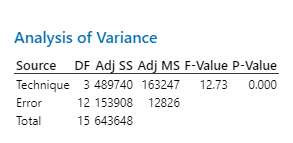
\includegraphics[width=0.5\textwidth]{./images/2_a.png}
    \caption{The output of the One-way ANOVA from Minitab.}
    \label{fig:2_a}
\end{figure}
Performing an F test at we can see that the P-value$ = 0.000 < \alpha = .05$, therefore we can conclude the following.
There is enough statistical evidence to support the hypothesis that not all means are equal.

\subsection*{b)}
\begin{figure}[h]
    \centering
    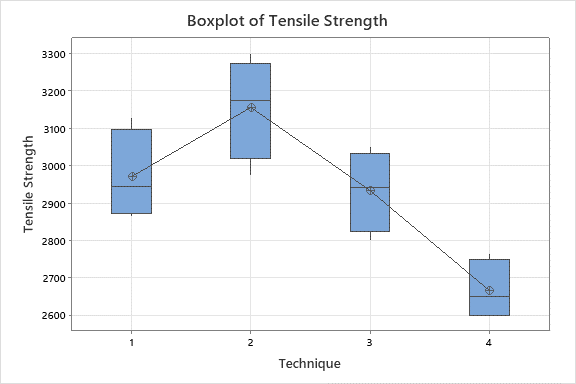
\includegraphics[width=1\textwidth]{./images/2_b.png}
    \caption{The Boxplot of tensile strength of the One-way ANOVA test from Minitab.}
    \label{fig:2_b}
\end{figure}
Judging by the boxplot alone, It would seem that the means are significantly different.
This is consistent with the above hypothesis test.
It looks as though the mean for treatment 1 and treatment 3 could be similar, in a pairwise comparison.
\subsection*{c)}
The results of the Fisher's LSD test can be summarized in the graphical results below.
Note that a line under the treatments indicates that they are not significantly different. \\
\vspace{12pt}
\\
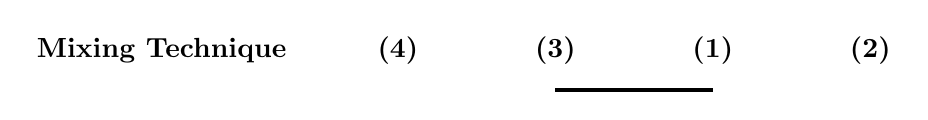
\begin{tikzpicture}[yscale=-1]
    % Define the positions of the labels
    \coordinate (labelPos) at (0, 0);
    \coordinate (4Pos) at (3, 0);
    \coordinate (3Pos) at (5, 0);
    \coordinate (1Pos) at (7, 0);
    \coordinate (2Pos) at (9, 0);

    % Draw the labels
    \node at (labelPos) {\textbf{Mixing Technique}}; % Treatment label
    \node at (4Pos) {\textbf{(4)}};
    \node at (3Pos) {\textbf{(3)}};
    \node at (1Pos) {\textbf{(1)}};
    \node at (2Pos) {\textbf{(2)}};

    % Draw the line
    \draw[ultra thick] ([yshift=0.5cm]3Pos) -- ([yshift=0.5cm]1Pos);
    % \draw[thick] ([yshift=1cm]1Pos) -- ([yshift=1cm]2Pos); % another theoretical line.
\end{tikzpicture}


\subsection*{d)}

\begin{figure}[h]
    \centering
    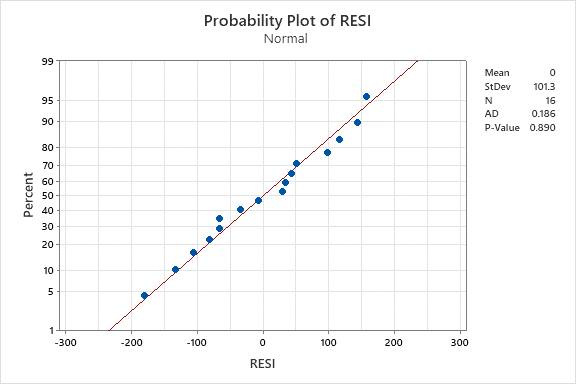
\includegraphics[width=1\textwidth]{./images/2_d.png}
    \caption{The normal probability plot of the residuals from Minitab.}
    \label{fig:2_d}
\end{figure}
\begin{flushleft}
$H_0$: The data are drawn from a normal disribution. \\
$H_a$: The data are not drawn from a normal disribution. \\
\end{flushleft}
Since the P-value is very large (0.890), we can conclude the following. 
The evidence of the data is consistent with the data being drawn from a normal disribution.

\subsection*{e)}
\begin{figure}[h]
    \centering
    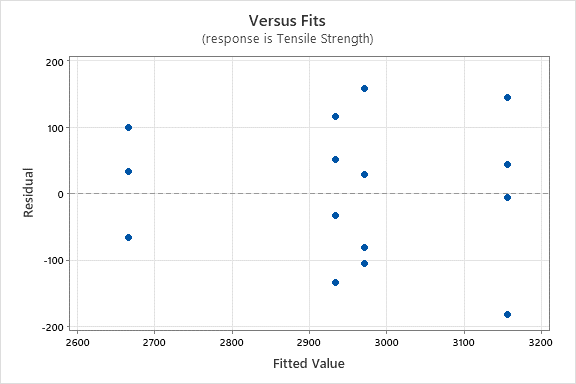
\includegraphics[width=1\textwidth]{./images/2_e.png}
    \caption{The residuals versus the predicted tensile strength from Minitab.}
    \label{fig:2_e}
\end{figure}
This graph indicates that there is not heteroskedasticity present,
that along with the conclusion that the data is drawn from
a normal distribution indicates that the model assumptions are verified
and the hypothesis test is valid.

\clearpage
\section*{Question 3}
\subsection*{a)}
Tukeys's test at $FWE\alpha = 0.05$ is as follows.
Note that there are $k = \binom{4}{2} = 6$ pairs, and the significance level is $\frac{\alpha}{k} = \frac{.05}{6} = 0.008\bar{3}$.
\begin{figure}[h]
  \centering
  
\includegraphics[width=1\textwidth]{./images/3.png}
  \caption{The output of the One-way ANOVA: Tensile Strength versus Technique at $\alpha = 0.0083$ from Minitab.}
  \label{fig:2_a}
\end{figure}

The graphical results are: \\
\vspace{12pt}
\\
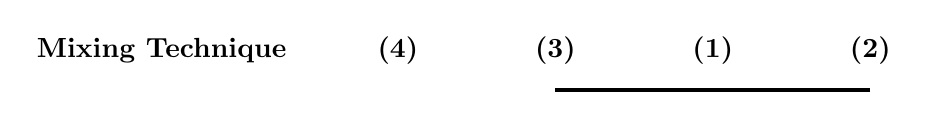
\begin{tikzpicture}[yscale=-1]
    % Define the positions of the labels
    \coordinate (labelPos) at (0, 0);
    \coordinate (4Pos) at (3, 0);
    \coordinate (3Pos) at (5, 0);
    \coordinate (1Pos) at (7, 0);
    \coordinate (2Pos) at (9, 0);

    % Draw the labels
    \node at (labelPos) {\textbf{Mixing Technique}}; % Treatment label
    \node at (4Pos) {\textbf{(4)}};
    \node at (3Pos) {\textbf{(3)}};
    \node at (1Pos) {\textbf{(1)}};
    \node at (2Pos) {\textbf{(2)}};

    % Draw the line
    \draw[ultra thick] ([yshift=0.5cm]3Pos) -- ([yshift=0.5cm]2Pos);
    % \draw[thick] ([yshift=1cm]1Pos) -- ([yshift=1cm]2Pos); % another theoretical line.
\end{tikzpicture} \\

These results are different from The Fisher LSD method as they indicate that technique 1, 2, and 3 are not not significantly different.


\clearpage
\section*{Question 4}
\subsection*{a)}
$H_0$: All means are equal. \\
$H_a$: Not all means are equal. \\
Performing an F test at we can see that the P-value $ = .052 > \alpha = .05$, therefore we can conclude the following.
The evidence from the data is consistent with the hypothesis that all means are equal.

\subsection*{b)}
Given that the F test concluded that all means are equal, It should not matter what fluid is selected given that the objective is long life.
That being said, if forced to choose, I would pick fluid 3, as it had the highest sample mean at $\bar{y}_{3 \cdot} = 20.95$.
\subsection*{c)}
\begin{figure}[h]
    \centering
    \begin{subfigure}[b]{0.4\textwidth}
        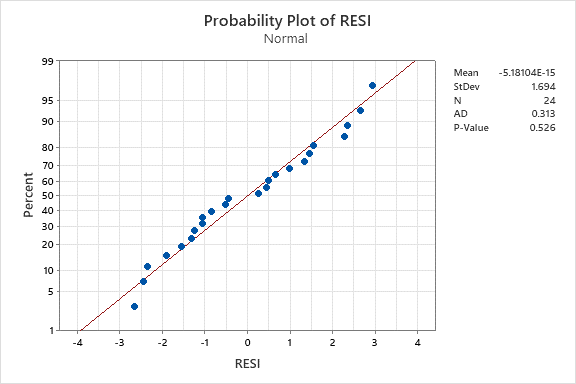
\includegraphics[width=1.25\textwidth]{./images/4_c_1.png}
        \caption{Minitab output showing normal probability plot.}
      \label{fig:img1}
    \end{subfigure}
    \hfill
    \begin{subfigure}[b]{0.4\textwidth}
        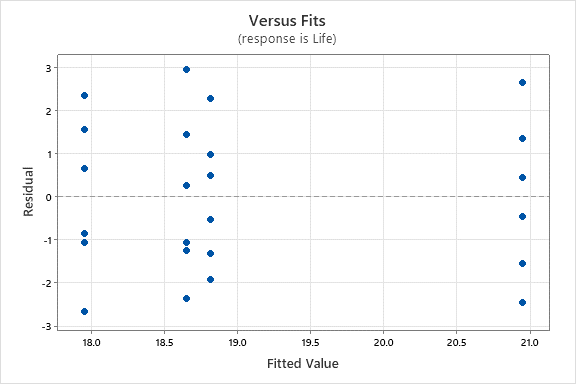
\includegraphics[width=1.25\textwidth]{./images/4_c_2.png}
        \caption{Minitab output showing the residuals vs fitted value.}
      \label{fig:img2}
    \end{subfigure}
    \label{fig:both}
\end{figure}

\begin{flushleft}
$H_0$: The data are drawn from a normal disribution. \\
$H_a$: The data are not drawn from a normal disribution. \\
\end{flushleft}
Performing an Anderson Darling normality test at $\alpha = 0.05$ on the residuals gives a P-value of 0.526.
Since the P-value is larger than $\alpha$, we can conclude the following. 
The evidence of the data is consistent with the data being drawn from a normal disribution.

Observing the residuals shows no indication of heteroskedasticity. This, along with the normality test indicates that the
basic analysis of variance assumptions are satisfied.
\subsection*{d)}
In order to test whether the average of the mean life of the two fluid types 1 and 3 is greater than the
mean life of fluid type 4. We set up the following right-tailed test at $\alpha = 0.05$.
\begin{flushleft}
  $H_0$: $\frac{1}{2}(\mu_1 + \mu_3) - \mu_4 = 0$ \\
  $H_a$: $\frac{1}{2}(\mu_1 + \mu_3) - \mu_4 > 0$ \\
\end{flushleft}
The contrast of intrest, where $c_1 = \frac{1}{2}, c_2 = 0, c_3 = \frac{1}{2}, c_4 = -1$, and $a = 4$ is:
\begin{align*}
    \hat{\Gamma} &=  \sum_{i=1}^{a} c_i \bar{y}_{i \cdot} \\
                &= \frac{1}{2}(18.65) + 0(17.95) + \frac{1}{2}(20.95) - (18.817) \\
                &= 0.983 
\end{align*}
Noting that $MSE = 3.3$, and $n = 6$ the test statistic is:
\begin{align*}
  t &=  \frac{\sum_{i=1}^{a} c_i \bar{y}_{i \cdot}}{\sqrt{\frac{MSE}{n} \cdot \sum_{i=1}^{a} c_i^2}} \\
              &= \frac{0.983}{\sqrt{\frac{3.3}{6} \cdot 1.5}} \\
              &= 1.032
\end{align*}
Since $t_{\alpha,N-a} = t_{.05,24-4} = 1.725$ the test is not in the right-tailed critical region, thus we can conclude the following.
There is not enough statistical evidence to support the hypothesis that the average of the mean life of the two fluid types 1 and 3 is greater than the
mean life of fluid type 4.

\subsection*{e)}
Bonferroni's method to do a pairwise comparison at $FWE\alpha = 0.05$ is as follows.
Note that there are $k = \binom{4}{2} = 6$ pairs, and the significance level is $\frac{\alpha}{k} = \frac{.05}{6} = 0.008\bar{3}$.
The test statistic, where $MSE = 3.3$, $n_i = n_j = 6$, and $N - a = 24 - 4 = 20$, is:
\begin{align*}
  t_{\alpha/2k , N-a} \sqrt{MSE(\frac{1}{n_i} + \frac{1}{n_j})}&=  t_{0.00069,20} \sqrt{3.3(\frac{1}{6} + \frac{1}{6})} \\
              &= 4.008 \sqrt{3.3(\frac{1}{6} + \frac{1}{6})} \\
              &= 4.203
\end{align*}
The differences, where
$\bar{y}_{1 \cdot} = 18.65$, $\bar{y}_{2 \cdot} = 17.95$, $\bar{y}_{3 \cdot} = 20.95$, and $\bar{y}_{4 \cdot} = 18.817$, are:
\begin{equation*}
  \begin{array}{c|c|c}
    \text{Difference} & \left|  \text{Difference} \right| & \text{Significantly Different?} \\
      \hline
      \bar{y}_{1 \cdot} - \bar{y}_{2 \cdot} & 0.700 & \text{No} \\
      \bar{y}_{1 \cdot} - \bar{y}_{3 \cdot} & 2.300 & \text{No} \\
      \bar{y}_{1 \cdot} - \bar{y}_{4 \cdot} & 0.167 & \text{No} \\
      \bar{y}_{2 \cdot} - \bar{y}_{3 \cdot} & 3.000 & \text{No} \\
      \bar{y}_{2 \cdot} - \bar{y}_{4 \cdot} & 0.867 & \text{No} \\
      \bar{y}_{3 \cdot} - \bar{y}_{4 \cdot} & 2.153 & \text{No} \\

  \end{array}
\end{equation*}\\
Therefore the graphical for Bonferroni's method to do a pairwise comparison are: \\
\vspace{12pt}
\\
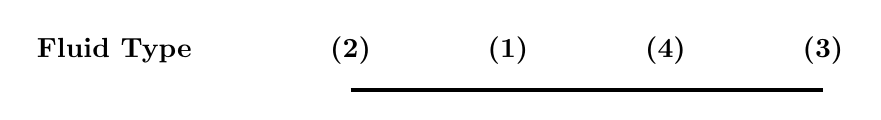
\begin{tikzpicture}[yscale=-1]
    % Define the positions of the labels
    \coordinate (labelPos) at (0, 0);
    \coordinate (2Pos) at (3, 0);
    \coordinate (1Pos) at (5, 0);
    \coordinate (4Pos) at (7, 0);
    \coordinate (3Pos) at (9, 0);

    % Draw the labels
    \node at (labelPos) {\textbf{Fluid Type}}; % Treatment label
    \node at (2Pos) {\textbf{(2)}};
    \node at (1Pos) {\textbf{(1)}};
    \node at (4Pos) {\textbf{(4)}};
    \node at (3Pos) {\textbf{(3)}};

    % Draw the line
    \draw[ultra thick] ([yshift=0.5cm]2Pos) -- ([yshift=0.5cm]3Pos);
    % \draw[thick] ([yshift=1cm]1Pos) -- ([yshift=1cm]2Pos); % another theoretical line.
\end{tikzpicture}


\clearpage
\section*{Question 5}
\subsection*{a)}
\begin{lstlisting}[language=R, 
    basicstyle=\ttfamily\small,
    numbers=none, 
    frame=single, 
    caption=R output of the summary of the aov function,
    label=code:cut-rod,
    escapeinside={(*}{*)}]
                Df Sum Sq Mean Sq F value Pr(>F)
    Brand        1   67.6    67.6   0.668  0.429
    Residuals   13 1315.7   101.2 
\end{lstlisting}
\begin{flushleft}
$H_0$: All means are equal. \\
$H_a$: Not all means are equal. \\
\end{flushleft}
Performing an F test at we can see that the P-value $ = 0.429 > \alpha = .05$, therefore we can conclude the following.
The evidence from the data is consistent with the hypothesis that all means are equal.
\subsection*{b)}
\begin{figure}[h]
    \centering
    \begin{subfigure}[b]{0.4\textwidth}
        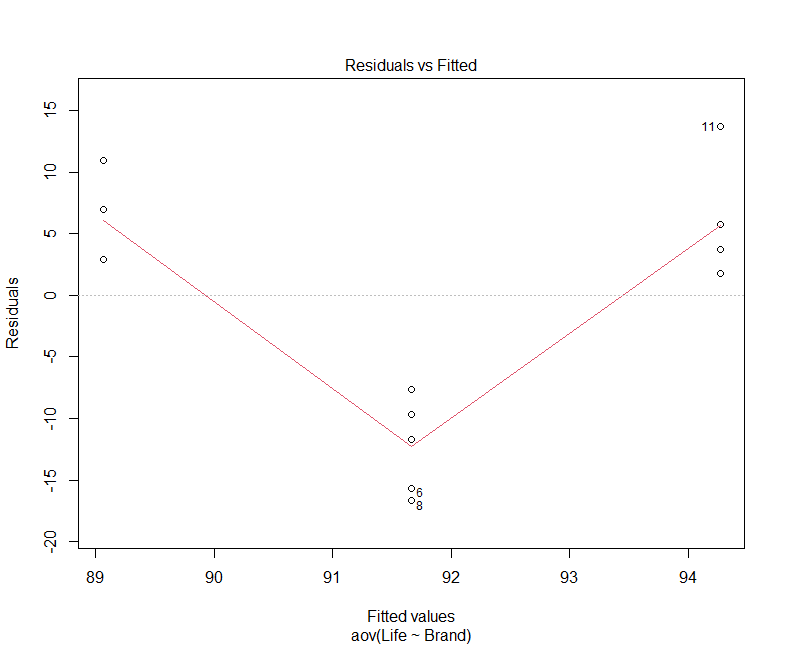
\includegraphics[width=1.25\textwidth]{./images/7_b_1.png}
        \caption{R output showing the residuals.}
      \label{fig:img1}
    \end{subfigure}
    \hfill
    \begin{subfigure}[b]{0.4\textwidth}
        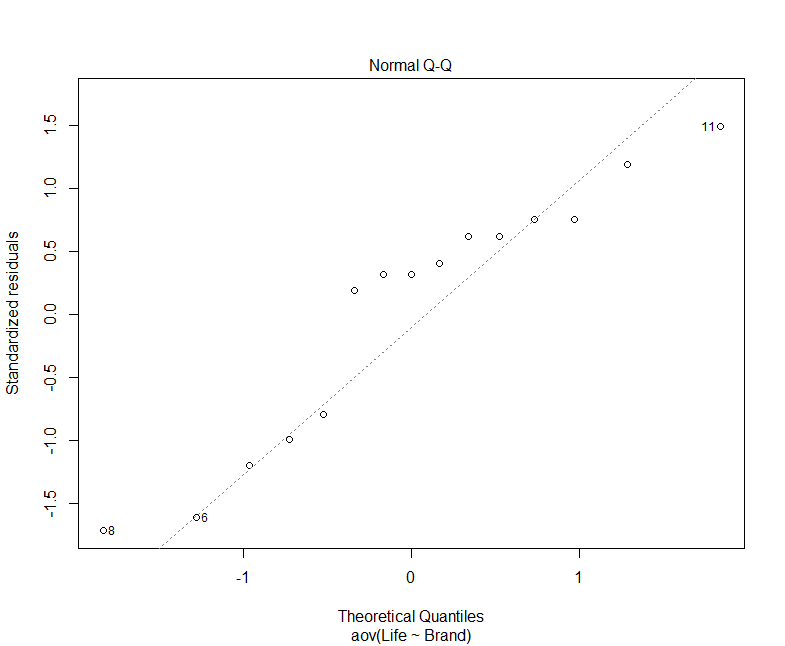
\includegraphics[width=1.25\textwidth]{./images/7_b_2.png}
        \caption{R output showing the normal probability plot.}
      \label{fig:img2}
    \end{subfigure}
    \label{fig:both}
\end{figure}

\clearpage
\subsection*{c)}
\subsubsection*{95 percent confidence interval estimate on
the mean life of battery brand 2.}
In order to construct a 95 percent confidence interval estimate on
the mean life of battery brand 2. The following equation can be used. \\
\begin{equation*}
    \sum_{i=1}^{a} c_i \bar{y}_{i \cdot} - t_{\alpha/2, N-a} \sqrt{\frac{MSE}{n} \sum_{i=1}^{a} c_i^2}
    \leq \sum_{i=1}^{a} c_i \mu_i \leq
    \sum_{i=1}^{a} c_i \bar{y}_{i \cdot} + t_{\alpha/2, N-a} \sqrt{\frac{MSE}{n} \sum_{i=1}^{a} c_i^2}
\end{equation*}
\begin{flushleft}
The contrast of intrest, where $c_1 = 0, c_2 = 1, c_3 = 0$, and $a = 3$ is:
\end{flushleft}
\begin{align*}
    \Gamma &=  \sum_{i=1}^{a} c_i \bar{y}_{i \cdot} \\
                &= 0(95.2) + 1(79.4) + 0(100.4) \\
                &= 79.4 
    \end{align*}
\begin{flushleft}
  Using R, the following values were obtained. $MSE = 1315.7$, and $t_{\alpha/2,N-a} = t_{0.025,12} = 2.178$.
  Thus, the 95 percent confidence interval estimate on
  the mean life of battery brand 2 is:
\end{flushleft}
\begin{align*}
  79.4 - 2.178 \sqrt{\frac{1315.7}{5} \cdot 1}
  &\leq \sum_{i=1}^{a} c_i \mu_i \leq
  79.4 + 2.178 \sqrt{\frac{1315.7}{5} \cdot 1} \\
  44.06
  &\leq \sum_{i=1}^{a} c_i \mu_i \leq
  114.73 \\
\end{align*}

\subsubsection*{99 percent confidence interval estimate on the mean difference between the lives of battery brands 2 and 3.}
The contrast of intrest, where $c_1 = 0, c_2 = 1, c_3 = -1$, and $a = 3$ is:
\begin{align*}
    \Gamma &=  \sum_{i=1}^{a} c_i \bar{y}_{i \cdot} \\
                &= 0(95.2) + 1(79.4) + -1(100.4) \\
                &= -21 
    \end{align*}
\begin{flushleft}
    Using R, the following values were obtained. $t_{\alpha/2,N-a} = t_{0.005,12} = 3.054$.
    Thus, the 99 percent confidence interval estimate on the mean difference between the lives of battery brands 2 and 3 is:
\end{flushleft}
\begin{align*}
    -21 - 3.054 \sqrt{\frac{1315.7}{5} \cdot 2}
    &\leq \sum_{i=1}^{a} c_i \mu_i \leq
    -21 + 3.054 \sqrt{\frac{1315.7}{5} \cdot 2} \\
    -91.06
    &\leq \sum_{i=1}^{a} c_i \mu_i \leq
    49.06 \\
\end{align*}
\subsection*{d)}
The percentage of batteries expected to fail before 85 weeks can be obtained in R using the following code.
\begin{lstlisting}[language=R, 
  basicstyle=\ttfamily\small,
  numbers=none, 
  frame=single, 
  caption=Calculating the percentage of batteries expected to fail before 85 weeks.,
  label=code:cut-rod,
  escapeinside={(*}{*)}]
  # Calculate percentage of batteries expected to fail
  percentage <- pnorm(85, mean = 100.4, sd = 36.27) * 100
  
  # Print the result
  percentage
\end{lstlisting}
\begin{lstlisting}[language=R, 
  basicstyle=\ttfamily\small,
  numbers=none, 
  frame=single, 
  caption=Code output.,
  label=code:cut-rod,
  escapeinside={(*}{*)}]
  33.5566
\end{lstlisting}


\clearpage
\section*{Question 6}
\begin{flushleft}
  $H_0$: $\sigma_1^2 = \sigma_2^2 = \sigma_3^2 = \sigma_4^2$. \\
  $H_a$: At least one $\sigma_i^2$ is different. \\
  \end{flushleft}
\begin{lstlisting}[language=R, 
  basicstyle=\ttfamily\small,
  numbers=none, 
  frame=single, 
  caption=R output of the bartlett test.,
  label=code:cut-rod,
  escapeinside={(*}{*)}]
	      Bartlett test of homogeneity of variances

  data:  Life by Fluid.Type
  Bartletts K-squared = 0.26691, df = 3,
  p-value = 0.9661
\end{lstlisting}
Since the P-value is large (0.9661), we fail to reject $H_0$, and can conclude the following.
There is not enough statistical evidence to support the hypotheis that at least one $\sigma_i^2$ is different.

This is the same conclusion met when observing the residual plot regarding equality of variances in question 4.

\section*{Question 7}
\begin{flushleft}
  $H_0$: $\sigma_1^2 = \sigma_2^2 = \sigma_3^2$. \\
  $H_a$: At least one $\sigma_i^2$ is different. \\
  \end{flushleft}
  \begin{figure}[h]
    \centering
    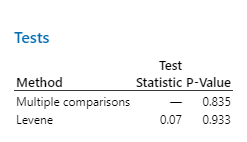
\includegraphics[width=0.5\textwidth]{./images/7.png}
    \caption{The output of the Test for Equal Variances: Life versus Brand from Minitab.}
    \label{fig:7}
\end{figure}
Since the P-value is large (0.933), we fail to reject $H_0$, and can conclude the following.
There is not enough statistical evidence to support the hypotheis that at least one $\sigma_i^2$ is different.

This is the same conclusion met when observing the residual plot regarding equality of variances in question 5.
\end{document}
